\section{Timing Compartments}
    Definition Here
    \subsection{ Applications }
    \subsubsection{ARM TrustZone}
    ARM TrustZone exemplifies a state of the practice solution that can enforce 
    a diverse range of security properties by restricting explicit information 
    flows between software modules. The security mechanisms of TrustZone may be 
    combined with the mechanisms proposed in this work to control both explicit 
    information flows and timing channels.

    \begin{figure}
        \begin{center}
            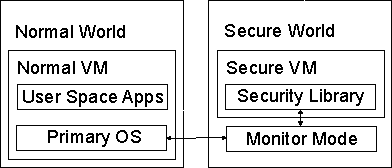
\includegraphics[width=3in]{figs/worlds.pdf}
            \caption{The explicit flow compartments of TrustZone-like 
            processor.}
            \label{fig:tz_domains}
        \end{center}
    \end{figure}

    TrustZone separates the software modules of a system into two explicit flow 
    compartments, the secure world and the normal world, as shown in Figure 
    \ref{fig:tz_domains}.
    This division minimizes the trusted computing base for some sensitive
    operations to a few small modules in the secure world.
    The first explicit flow compartment is called the normal world and it has a 
    virtual processor that contains the operating system and all user-space 
    applications. The other explicit flow compartment, the secure world, 
    contains a virtual processor that contains only a small execution 
    environment and a set of very simple libraries for handling protected 
    operations. This secure world virtual processor does not contain a complete 
    operating system and the libraries do not require any operating system 
    support (e.g. they may not have system calls). The secure world also 
    contains a software module called the monitor mode that handles context switching 
    between the two compartments if they are time multiplexed on the same core.

    The security levels of these compartments form a lattice such that the 
    level of the normal world precedes the level of the secure world (i.e. 
    information available to the normal world is available to the secure 
    world). All of the secure world code is small to reduce the chance of 
    vulnerabilities. The secure world must only allow the normal world to play 
    the video if the subscription is valid. It is worth noting that the normal 
    world OS is not trusted by the secure world and the secure world does not 
    depend on any support from the normal world OS.


    \begin{figure}
        \begin{center}
            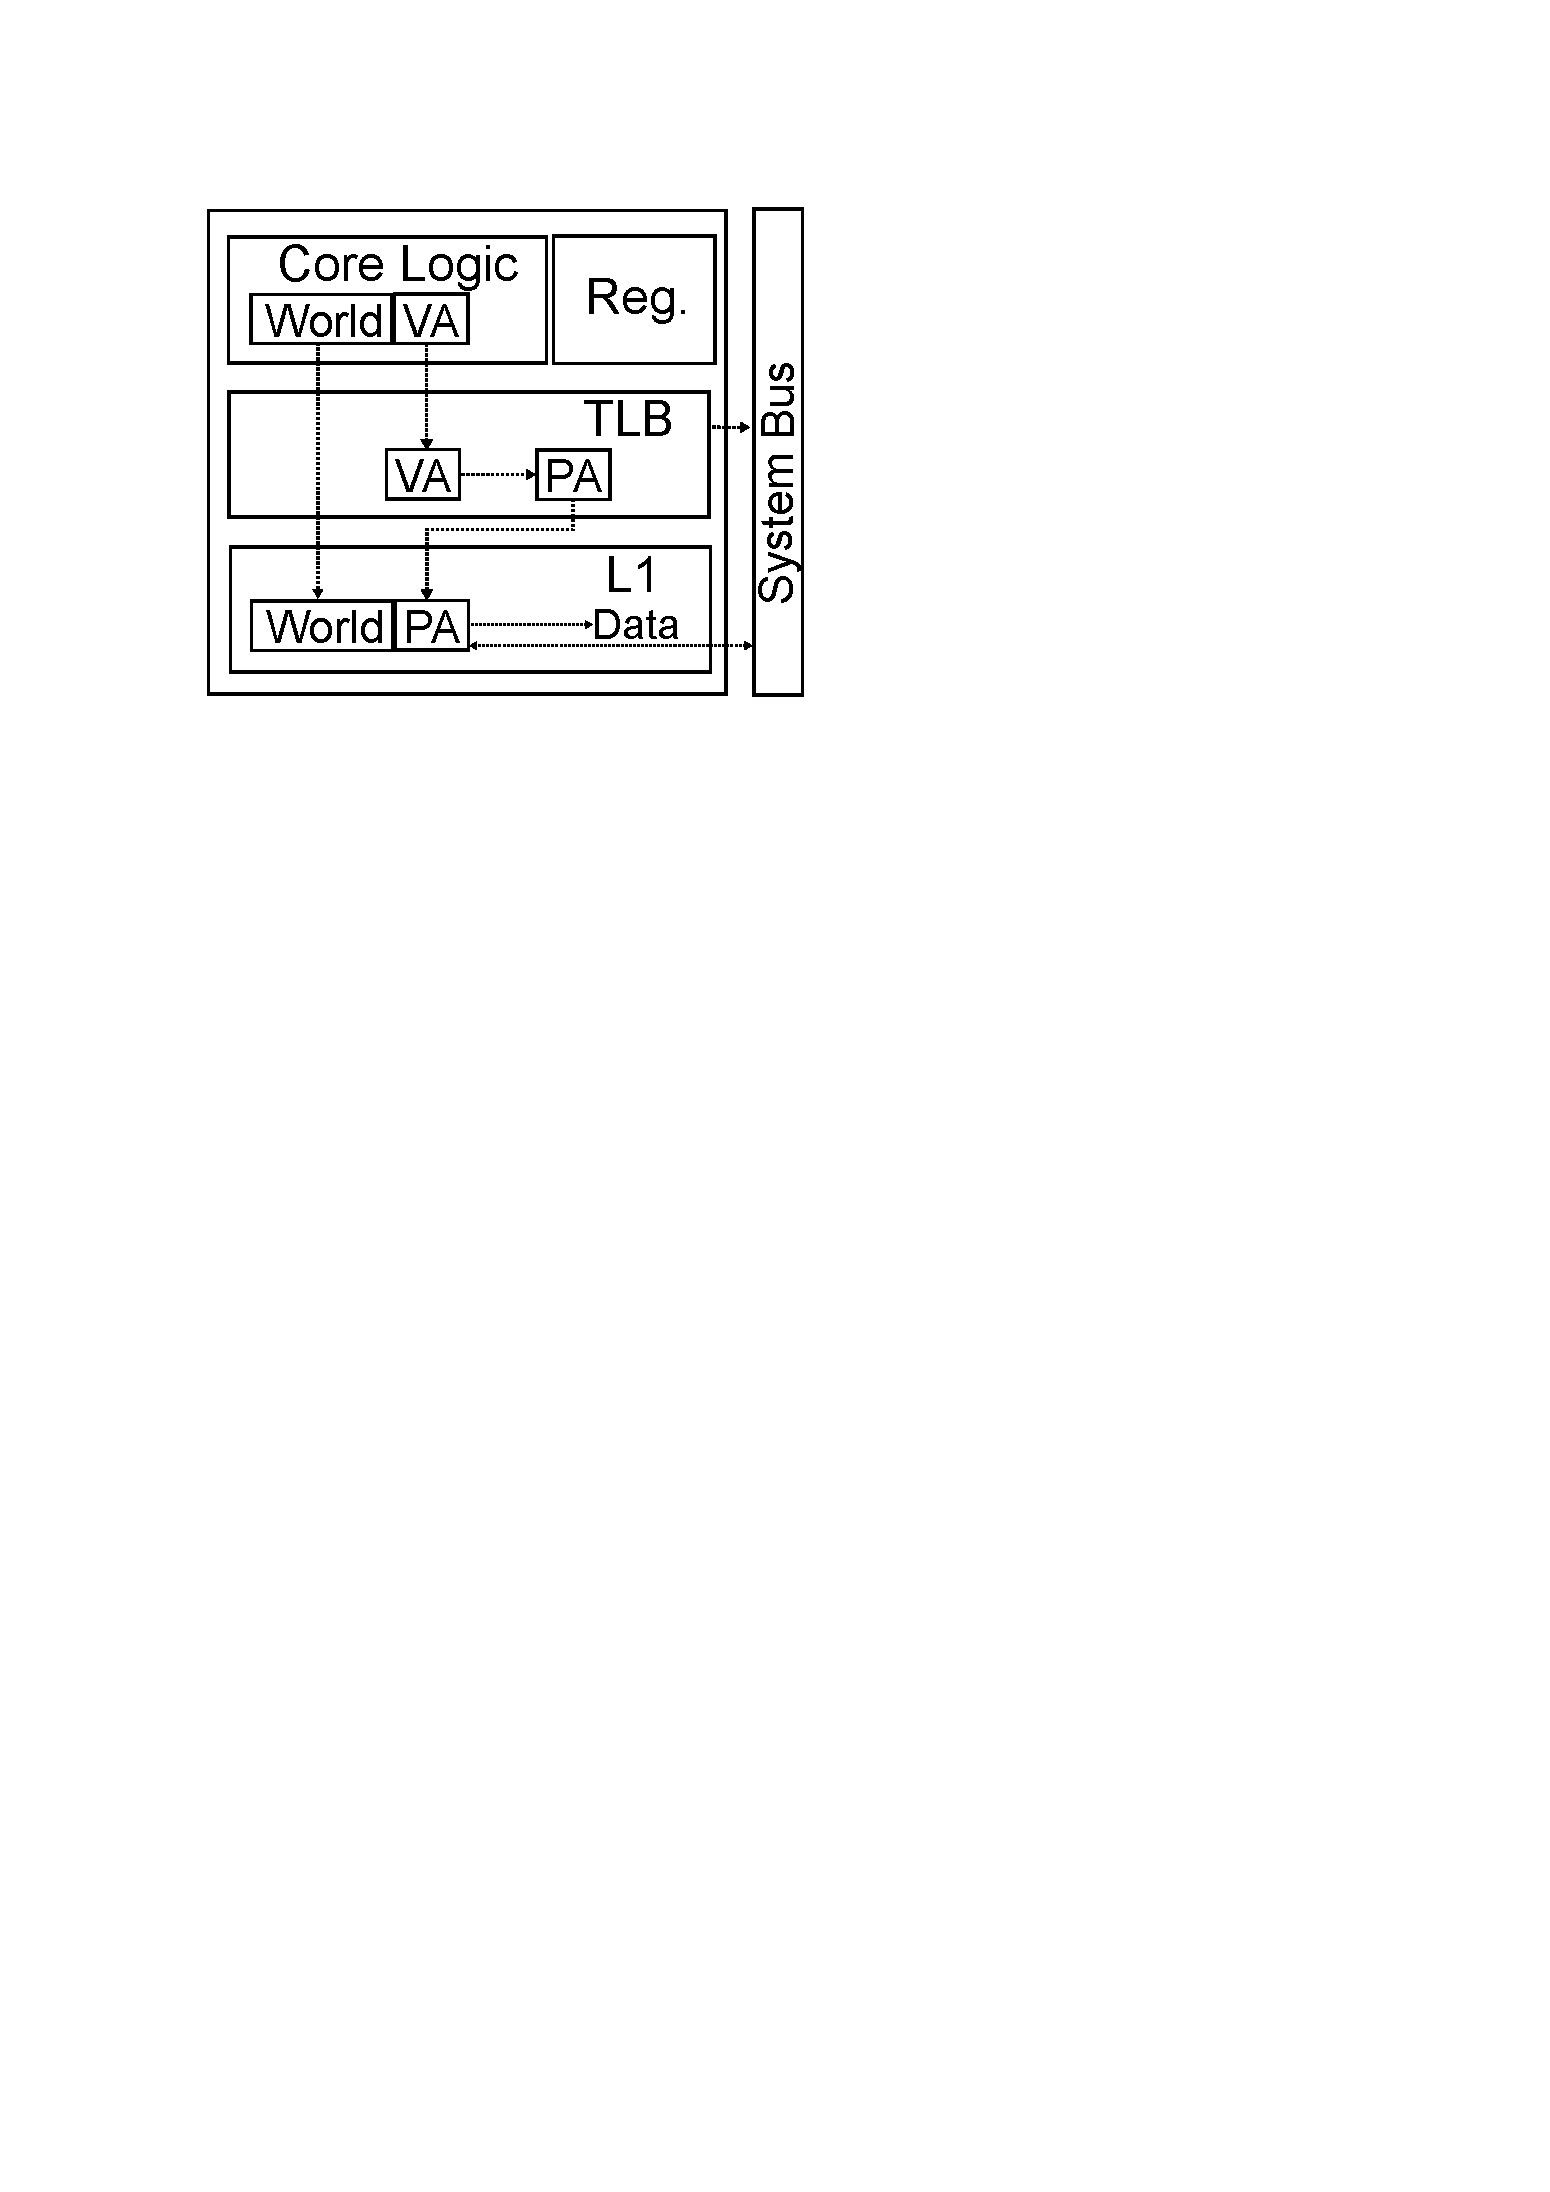
\includegraphics[width=3in]{figs/tz_tags.pdf}
            \caption{DRM Protection Mechnamisms. The baseline architecture is 
            extended with tags that control explicit information flows between 
        the secure and normal worlds.}
            \label{fig:tz_uarch}
        \end{center}
    \end{figure}

    TrustZone extends the baseline cores of Figure \ref{fig:baseline} to
    those shown in Figure \ref{fig:tz_uarch}. The core logic contains a tag to 
    store which compartment is currently executing. Each cache entry has a tag to 
    indicate if the entry can be accessed by the normal world compartment or not. To make 
    an access to the memory hierarchy, the core sends the virtual address and 
    the current compartment to the TLB. The TLB gets the physical address as normal 
    (performing a page table walk if needed). The physical address and current 
    explicit flow compartment are sent to the cache. If the cache contains the 
    physical address and the tag of the entry indicates that the current 
    compartment 
    has sufficient rights to accesss the entry, the access proceeds normally.  
    Otherwise, if it is a cache miss, the cache sends the physical address and 
    the current compartment to the system bus to access the main memory. If the tag 
    of the address in main memory indicates that the current compartment has 
    sufficient rights, the cache block is brought into the cache as normal and 
    the tag is set in the cache. If it is either a hit or a miss and the 
    security level does not meet the requirements, the access fails.

    The two virtual processors may share the same physical processor in 
    time-multiplexed way through context switching. Context switches between 
    these virtual processors are entered by a special instruction that invokes 
    the monitor mode.  Typically, the monitor mode will save the general 
    purpose registers and any processor configuration registers. The TLB and 
    caches are not flushed since the tags protect illegal data accesses.

